The collaborative side of the algorithm starts by receiving a single user, and afterwards get all different users put into a collection. With the IndexUsers method, there will be created a dictionary, which contains pairs of a user from the collection, together with a coefficient, based on the linear similarity between them and the main user. This coefficient is based on the Pearson correlation coefficient which has previously been described.

The two sets which is needed for each Pearson calculation, is the ratings of media items, which both the main user and secondary user have in common in their medialists. The Pearson calculation will then return a coefficient based on these two collections of ratings, indicating how similar they are in their ratings, and general rating habits. Following this, users with negative or no correlation will be removed, and the remaining is sorted by their given coefficient, going from highest to lowest. See figure [REF] for the Pearson calculation.
\begin{table}[htb]
\centering
\begin{tabular}{|l|l|l|l|l|} \hline
	\textbf{X} & \textbf{Y} & \textbf{XY}
	& \textbf{X2} & \textbf{Y2} \\ \hline
	2 & 3 & 6 & 4 & 9 \\ \hline
	4 & 5 & 20 & 16 & 25 \\ \hline
	6 & 5 & 56 & 64 & 49 \\ \hline\hline
	20 & 20 & 112 & 120 & 108 \\ \hline
\end{tabular}
\caption{Pearson Example}
\label{PearsonEx}
\end{table} 

In the above Table \ref{PearsonEx} is two sets of ratings, x and y, which is then put together to create 5 sums, which also can be seen above. These sums is then used as the parameters for the Pearson calculation, together will the number of pairs, which is 4. In this example Pearson will return 0,949, which is a very good coefficient.

The next part of the algorithm will take this sorted dictionary of users and coefficients, and begin extracting media for recommendations. It will start by looking at the user with the highest coefficient, and take media items which the main user does not have in their medialist, and the secondary user have rated higher than a certain threshold. Furthermore, if the same media occurs in other users medialists, it will receive a boost, putting it higher in the list. The same happens if the media was a friends medialist. See Figure \ref{CollaEx} for an illustration of this.

\begin{figure}[htb]
\centering
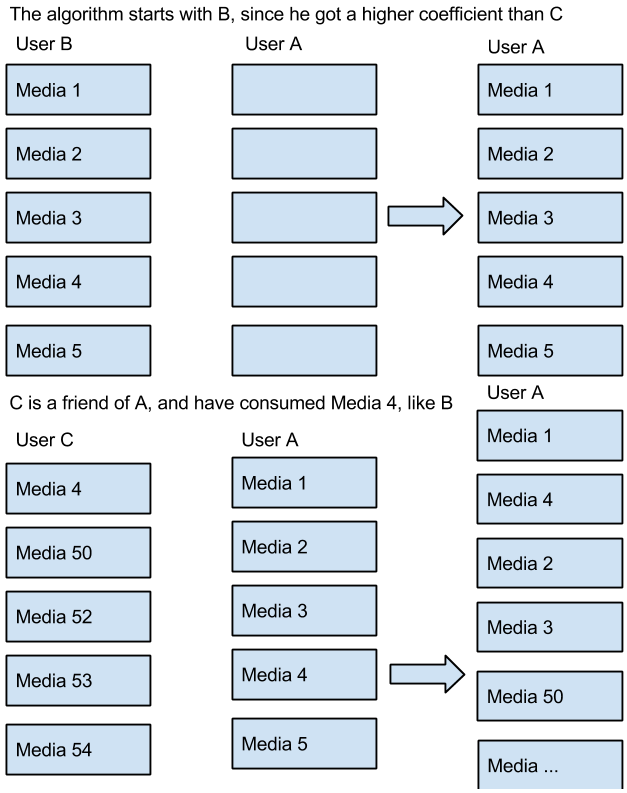
\includegraphics[width=0.8\textwidth]{Images/CollaborativeRecExample.png}
\caption{Example showing the collaborative selection process}
\label{CollaEx}
\end{figure}